%!TEX program = xelatex
\documentclass[12pt, a4paper]{article}

\usepackage[dvipsnames]{xcolor}

\usepackage{fancyhdr}
\usepackage{extramarks}
\usepackage{amsmath}
\usepackage{amsthm}
\usepackage{amsfonts}
\usepackage{tikz}
\usepackage[plain]{algorithm}
\usepackage{algpseudocode}

\usepackage{ctex}
\usepackage{indentfirst}
\usepackage{wrapfig}
\usepackage{upgreek}
\usepackage{subfigure}
\ctexset {today=old}
\usetikzlibrary{automata,positioning,shapes.geometric,arrows.meta,patterns,calc}
\numberwithin{equation}{section}

%
% Basic Document Settings
%

\topmargin=-0.25in
\evensidemargin=0in
\oddsidemargin=0in
\textwidth=6.5in
\textheight=9.2in
\headsep=0.25in

\linespread{1.1}

\pagestyle{fancy}
\lhead{\hmwkAuthorName}
\chead{\hmwkClass : \hmwkTitle}
\rhead{\firstxmark}
\lfoot{\lastxmark}
\cfoot{\thepage}

\renewcommand\headrulewidth{0.4pt}
\renewcommand\footrulewidth{0.4pt}

\setlength{\parindent}{2em}  % 2em代表首行缩进两个字符

%
% Create Problem Sections
%

\newcommand{\enterProblemHeader}[1]{
    \nobreak\extramarks{}{Problem \arabic{#1} continued on next page\ldots}\nobreak{}
    \nobreak\extramarks{Problem \arabic{#1} (continued)}{Problem \arabic{#1} continued on next page\ldots}\nobreak{}
}

\newcommand{\exitProblemHeader}[1]{
    \nobreak\extramarks{Problem \arabic{#1} (continued)}{Problem \arabic{#1} continued on next page\ldots}\nobreak{}
    \stepcounter{#1}
    \nobreak\extramarks{Problem \arabic{#1}}{}\nobreak{}
}

% \setcounter{secnumdepth}{0}
\newcounter{partCounter}
\newcounter{homeworkProblemCounter}
\setcounter{homeworkProblemCounter}{0}
% \nobreak\extramarks{Problem \arabic{homeworkProblemCounter}}{}\nobreak{}

%
% Homework Problem Environment
%
% This environment takes an optional argument. When given, it will adjust the
% problem counter. This is useful for when the problems given for your
% assignment aren't sequential. See the last 3 problems of this template for an
% example.
%
\newenvironment{homeworkProblem}[1][-1]{
    \ifnum#1>0
        \setcounter{homeworkProblemCounter}{#1}
    \fi
    \section{Problem \arabic{homeworkProblemCounter}}
    \setcounter{partCounter}{1}
    \enterProblemHeader{homeworkProblemCounter}
}{
    \exitProblemHeader{homeworkProblemCounter}
}

%
% Homework Details
%   - Title
%   - Due date
%   - Class
%   - Section/Time
%   - Instructor
%   - Author
%

\newcommand{\hmwkTitle}{Mechanical Vibration}
\newcommand{\hmwkDueDate}{\today}
\newcommand{\hmwkClass}{University Physics}
\newcommand{\hmwkClassTime}{}
\newcommand{\myUniversiy}{Wuhan University}
\newcommand{\hmwkAuthorName}{\textbf{Lai Wei}}

%
% Title Page
%

\title{
    \vspace{2in}
    \textmd{\textbf{\hmwkClass:\ \hmwkTitle}}\\
    \normalsize\vspace{0.1in}\small{Date: \hmwkDueDate}\\
    \vspace{0.1in}\large{\textit{\myUniversiy}}
    \vspace{3in}
}

\author{\hmwkAuthorName}
\date{}

\renewcommand{\part}[1]{\textbf{\large Part \Alph{partCounter}}\stepcounter{partCounter}\\}

%
% Various Helper Commands
%

% Useful for algorithms
\newcommand{\alg}[1]{\textsc{\bfseries \footnotesize #1}}

% % For derivatives
% \newcommand{\deriv}[1]{\frac{\mathrm{d}}{\mathrm{d}x} (#1)}

% For partial derivatives
\newcommand{\pderiv}[2]{\frac{\partial}{\partial #1} (#2)}

% Integral dx
\newcommand{\dx}{\mathrm{d}x}

% Alias for the Solution section header
\newcommand{\solution}{\textbf{\large Solution}}

% Probability commands: Expectation, Variance, Covariance, Bias
\newcommand{\E}{\mathrm{E}}
\newcommand{\Var}{\mathrm{Var}}
\newcommand{\Cov}{\mathrm{Cov}}
\newcommand{\Bias}{\mathrm{Bias}}

% 我的newcommand
\newcommand{\degree}{^{\circ}}
\newcommand{\arrow}{-{Stealth[length=4mm,width=2mm]}}
\newcommand{\rmd}{\mathrm{~d}}
\newcommand{\deriv}[2]{\frac{\rmd #1}{\rmd #2}}
\renewcommand{\parallel}{\mathrel{/\mskip-2.5mu/}}

\begin{document}

\maketitle

\pagebreak

% 设置页码格式是罗马数字
\pagenumbering{roman}

% 生成目录
\tableofcontents

\newpage 
\mbox{}
\newpage

\pagebreak

% 设置页码格式是阿拉伯数字
\pagenumbering{arabic}

\pagebreak

    机械振动:物体围绕一固定位置往复运动。

\section{简谐振动}

\subsection{简谐振动的动力学特征}

\subsubsection{弹簧振子的振动}

    模型:谐振子轻弹簧(不计质量)与物体(看成质点)

    弹簧振子的无阻尼自由振动:

    \[
        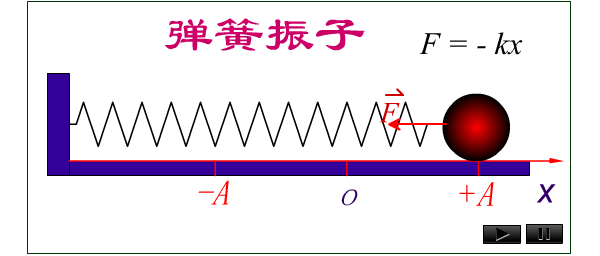
\includegraphics[scale=0.5]{Chapter 06 images/pic1.png}
    \]

    振动的成因:

    \begin{enumerate}
        \item 回复力;
        \item 惯性。
    \end{enumerate}

\subsubsection{弹簧振子的运动方程}

    \begin{equation}
        F=-k x=m a=m \frac{\rmd^2 x}{\rmd t^2}
    \end{equation}

    令
    
    \[
        \omega^2=\frac{k}{m}
    \]
    
    得
    
    \[
        \dfrac{\rmd^2 x}{\rmd t^2} = -\omega^2 x
    \]

    即\(a=-\omega^2 x\)

    具有加速度\(a\)与位移的大小\(x\)成正比,而方向相反特征的振动称为简谐运动。

    简谐运动的微分方程:

    \begin{align}
        \dfrac{\rmd^2 x}{\rmd t^2} = -\omega^2 x
    \end{align}

    解得

    \begin{align}
        x = A \cos\left(\omega t + \varphi\right)
    \end{align}

    或

    \begin{align}
        x = A \sin\left(\omega t + \varphi + \frac{\uppi}{2}\right)
    \end{align}

    用复指数表示
    
    \begin{equation}
        x=A \mathrm{e}^{\mathrm{i}(\omega t+\varphi)}
    \end{equation}

    \textbf{公式之间的相互推导关系}

    \[
        \tikzset{every picture/.style={line width=0.75pt}} %set default line width to 0.75pt
        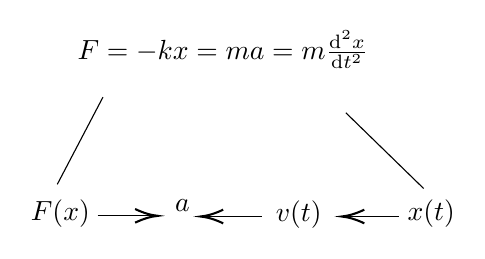
\begin{tikzpicture}[x=0.75pt,y=0.75pt,yscale=-1,xscale=1]
            %uncomment if require: \path (0,300); %set diagram left start at 0, and has height of 300
            %Straight Lines [id:da5445518985427571] 
            \draw    (155.43,153.29) -- (182.43,153.29) ;
            \draw [shift={(184.43,153.29)}, rotate = 180] [color={rgb, 255:red, 0; green, 0; blue, 0 }  ][line width=0.75]
                (10.93,-3.29) .. controls (6.95,-1.4) and (3.31,-0.3) .. (0,0) .. controls (3.31,0.3) and (6.95,1.4) .. (10.93,3.29)   ;
            %Straight Lines [id:da8539578247281134] 
            \draw    (234.5,153.61) -- (207,153.61) ;
            \draw [shift={(205,153.61)}, rotate = 360] [color={rgb, 255:red, 0; green, 0; blue, 0 }  ][line width=0.75]
                (10.93,-3.29) .. controls (6.95,-1.4) and (3.31,-0.3) .. (0,0) .. controls (3.31,0.3) and (6.95,1.4) .. (10.93,3.29)   ;
            %Straight Lines [id:da08053806804260755] 
            \draw    (300.5,153.61) -- (275,153.61) ;
            \draw [shift={(273,153.61)}, rotate = 360] [color={rgb, 255:red, 0; green, 0; blue, 0 }  ][line width=0.75]
                (10.93,-3.29) .. controls (6.95,-1.4) and (3.31,-0.3) .. (0,0) .. controls (3.31,0.3) and (6.95,1.4) .. (10.93,3.29)   ;
            %Straight Lines [id:da2022111052056348] 
            \draw    (158,96.11) -- (136,138.11) ;
            %Straight Lines [id:da9851232959428675] 
            \draw    (275,103.61) -- (312.5,140.11) ;
            % Text Node
            \draw (122,144.4) node [anchor=north west][inner sep=0.75pt]    {$F( x)$};
            \draw (191.5,144.4) node [anchor=north west][inner sep=0.75pt]    {$a$};
            \draw (240,144.9) node [anchor=north west][inner sep=0.75pt]    {$v( t)$};
            \draw (303.5,144.4) node [anchor=north west][inner sep=0.75pt]    {$x( t)$};
            \draw (144.5,62.9) node [anchor=north west][inner sep=0.75pt]    {$F=-kx=ma=m\frac{\mathrm{d}^{2} x}{\mathrm{d} t^{2}}$};
        \end{tikzpicture}
    \]

\subsubsection{谐振动的速度和加速度}

    由

    \begin{align*}
        x = A \cos\left(\omega t + \varphi\right)
    \end{align*}

    运动方程对时间求导

    \begin{equation}
        v=\frac{\mathrm{d} x}{\mathrm{~d} t}=-\omega A \sin (\omega t+\varphi)=-v_{\mathrm{m}} \sin (\omega t+\varphi)
    \end{equation}

    运动方程对时间求二阶导

    \begin{equation}
        a=\frac{\mathrm{d}^2 x}{\mathrm{~d} t^2}=-\omega^2 A \cos (\omega t+\varphi)=
        -a_{\mathrm{m}} \cos (\omega t+\varphi)
    \end{equation}

    其中,

    $$
        A=\sqrt{x_0^2+\left(\frac{v_0}{\omega}\right)^2}
    $$

    $$
        \varphi=\arctan \left(-\frac{v_0}{\omega x_0}\right)
    $$

    (此结果一般有两个值,最后要舍去一个,根据速度的方向。)
    
    \[
        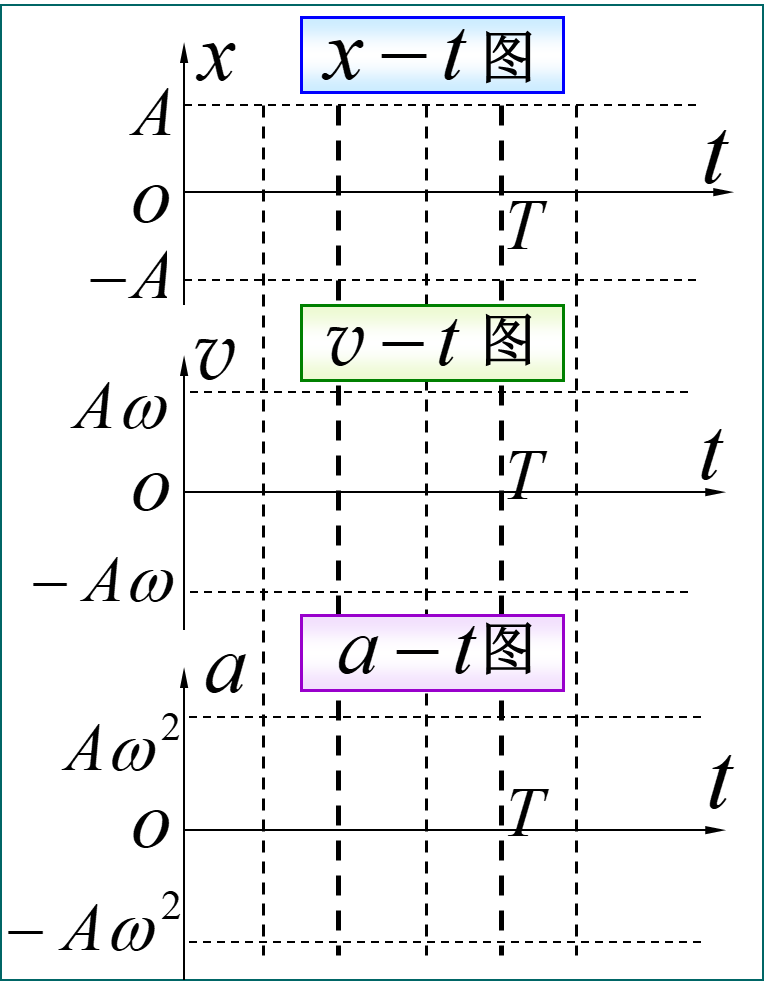
\includegraphics[scale=0.5]{Chapter 06 images/pic2.png}
    \]

\subsubsection{描述简谐振动的物理量}

    振幅 (amplitude):

    \begin{align}
        x_m = A
    \end{align}

    周期 (period):

    \begin{align}
        T = \frac{2 \uppi}{\omega}
    \end{align}

    简谐运动中,\(\omega\)被称为角频率或圆频率

    \begin{align}
        \omega = \sqrt{\frac{k}{m}}
    \end{align}

    频率 (frequency):

    \begin{align}
        \nu = \frac{1}{T}
    \end{align}

    相位 (phase):

    \begin{align}
        \left(\omega t + \varphi\right)
    \end{align}

    初相位(初相,initial phase)

    \begin{align}
        \varphi
    \end{align}

    相位差:

    设有两个同方向、同频率的简谐振动,它们的振动表达式分别为
    
    $$
        \begin{aligned}
            & x_1=A_1 \cos \left(\omega t+\varphi_1\right) \\
            & x_2=A_2 \cos \left(\omega t+\varphi_2\right)
        \end{aligned}
    $$

    它们在任意时刻的相位差为

    \begin{align}
        \Delta \varphi = \left(\omega t+\varphi_1\right) - \left(\omega t+\varphi_2\right)
    \end{align}

\end{document}
